% ----------------------------------------------------------------------
% Nobby compatible default settings. Make sure you document features
% all of the packages and definitions between here and the 'Optional'
% section.
% 
% 11pt and 12pt fonts usually work but may exhibit errors in
% conjunction with the --scale option.
% 
% Use documentclasses other than 'article' at your own risk.
% 
% ----------------------------------------------------------------------
\documentclass[10pt]{article}
\usepackage{amsmath, amsthm, amssymb}
\usepackage[latin1]{inputenc}
\usepackage{graphicx}

% Nobby will copy the title and author as comments into the HTML file.
\title{Nobby Demo}
\author{Oliver Nagy (olitheolix@gmail.com)}

% Define default theorem environments. If you define additiona onses,
% eg. '\newtheorem{foo}{Foo}', be sure to add 'foo' to
% 'config.counter_names'.
\newtheorem{lemma}{Lemma}
\newtheorem{theorem}{Theorem}
\newtheorem{example}{Example}
\newtheorem{corollary}{Corollary}
\newtheorem{definition}{Definition}

% ----------------------------------------------------------------------
% Optional
% 
% Include- and define your own packages and macros here, set LaTeX
% counters, modify variables, etc.
% ----------------------------------------------------------------------
\usepackage{parskip}
\usepackage{tikz}
\usetikzlibrary{calc, through, arrows}
\usepackage{subcaption}
\usepackage[pdftex,bookmarks=true, pdftitle={Nobby Demo},
pdfauthor={Oliver Nagy}, colorlinks=true,
citecolor=black, linkcolor=black]{hyperref}

% Custom macro.
\newcommand{\mvec}[1]{\mathbf{#1}}

% ----------------------------------------------------------------------
% Do not (re)define macros, environments, counters, variables,
% etc. beyond this point.
% ----------------------------------------------------------------------
\begin{document}
\maketitle

\section{Outline}
\label{sec:one}
This file demonstrates some of the constructs Nobby can convert to
HTML. Nobby relies on properly formatted \LaTeX code to do its work
properly.

Here is Pythagoras' theorem in an \emph{align} environment:
\begin{align}
  \label{eq:pyth}
  z = \sqrt{x^2 + y^2}.
\end{align}
Here it is again as an inline formula: $z = \sqrt{x^2 + y^2}$.

Nobby automatically escapes the <> characters. It is therefore safe to
write <strong> or </strong> without accidentally inserting HTML tags.

Similarly, Nobby also translate quotes: ``text in quotes'' and
escaped \LaTeX symbols like ``\$'', ``\{``, ``\}'' and ``\%'' to
proper HTML, ie. without the leading backslash.


\subsection{More formatting}
You can, of course, \emph{emphasise} something.

Inline math expressions like $x=1$ or $e^{i\pi} + 1 = 0$ work fine.

Here is some plain text. {{This sentence is actually an SVG image.}}

The \texttt{\textbackslash{ldots}} command is often useful\ldots as is the
\texttt{typewriter font}, or a \textbf{bold} statement.

\subsection{Environments}
Nobby does not know about \LaTeX macros or environments. It converts
them to images unless a plugin exists for them. The following examples
demonstrate some of the default plugins.

\subsubsection{Itemize}
\begin{itemize}
\item Item 1
\item Item 2
\end{itemize}

\subsubsection{Enumerate}
\begin{enumerate}
\item Item 1
\item Item 2
\end{enumerate}

\subsubsection{Equation}
\begin{equation}
  \label{eq:rel}
  E = mc^2.
\end{equation}

\subsubsection{Theorem Envoronments}
The AMS package provides way to define theorem environments with
\texttt{\textbackslash{newtheorem\{theorem\}\{Theorem\}}}. Nobby
assumes that ``lemma'', ``theorem'', ``example'', ``corollary'' and
``definition'' are defined the document preamble. The HTML conversion
will fail if not.

Nobby ships with a single plugin to handle all these theorem
environments. Here are some examples.

Compare the quality of this version with the 
\href{http://en.wikipedia.org/wiki/Divergence_theorem}{original} on
Wikipedia).
\begin{theorem}[Divergence Theorem]
  \label{thm:div}
  Suppose $\mathcal{V}$ is a subset of $\mathbb{R}^n$ (in the case of
  $n=3$, $\mathcal{V}$ represents a volume in 3D space) which is
  compact and has a piecewise smooth boundary $\mathcal{S}$ (also
  indicated with $\partial\mathcal{V} = \mathcal{S}$). If $F$ is a
  continuously differentiable vector field defined on a neighborhood
  of $\mathcal{V}$, then we have
  \begin{align}
    \iiint_{\mathcal{V}} \nabla \cdot F(\mvec{v})\; \textnormal{d}\mvec{v}
    = \oint_{\mathcal{S}} F(\mvec{s})\; \textnormal{d}\mvec{s}.
  \end{align}
\end{theorem}

Another one from \href{http://en.wikipedia.org/wiki/Divergence}{Wikipedia}:
\begin{definition}[Divergence in Cartesian Coordinates]
  \label{def:div}
  Let $x, y, z$ be a system of Cartesian coordinates in 3-dimensional
  Euclidean space, and let $i, j, k$ be the corresponding basis of unit
  vectors. The divergence of a continuously differentiable vector
  field $F = U i + V j + W k$ is equal to the scalar-valued function:
  \begin{align}
    \textnormal{div } F = \nabla \cdot F = 
    \frac{\partial U}{\partial x} +
    \frac{\partial V}{\partial y} +
    \frac{\partial W}{\partial z}.
  \end{align}
\end{definition}

Here is yet another definition from Wikipedia to demonstrate the
continuous enumeration of theorem environments and equations
therein. The definition also references its own equations. The
following definition of the Laplacian is from
\href{http://en.wikipedia.org/wiki/Laplace_operator}{here}.
\begin{definition}[Laplace Operator]
  \label{def:lap}
  The Laplace operator is a second order differential operator in the
  $n$-dimensional Euclidean space, defined as the divergence
  ($\nabla\cdot$) of the gradient ($\nabla f$). Thus if $f$ is a
  twice-differentiable real-valued function, then the Laplacian of $f$
  is defined by
  \begin{align}
    \label{eq:lapdef1}
    \Delta f = \nabla^2f = \nabla\cdot\nabla f
  \end{align}
  where the latter notations derive from formally writing $\nabla =
  \left(\frac{\partial}{\partial x_1}, \ldots,
    \frac{\partial}{\partial x_n}\right)$. Equivalently, the Laplacian
  of $f$ is the sum of all the unmixed second partial derivatives in the
  Cartesian coordinates
  \begin{align}
    \label{eq:lapdef2}
    \Delta f = \sum_{i=1}^n \frac{\partial^2f}{\partial x_i^2}
  \end{align}
  As a second-order differential operator, the Laplace operator maps
  $C^k$-functions to $C^{k-2}$-functions for $k\geq 2$. The expression
  (\ref{eq:lapdef1}) (or equivalently (\ref{eq:lapdef2})) defines an
  operator $\Delta : C^k(\mathbb{R}^n) \mapsto
  C^{k-2}(\mathbb{R}^n)$, or more generally an operator $\Delta :
  C^k(\Omega) \mapsto C^{k-2}(\Omega)$ for any open set $\Omega$.
\end{definition}

You can numerically reference Theorem \ref{thm:div}, Definition
\ref{def:div} and Definition \ref{def:lap} as usual. Alternatively,
you may also reference them with the \texttt{\textbackslash{hyperref}}
macro and link directly to the \hyperref[thm:div]{Divergence Theorem},
the \hyperref[def:div]{Definition of Divergence}, or the
\hyperref[def:div]{Definition of the Laplacian}.

\begin{theorem}
  \label{thm:no_largest_int}
  There is no largest integer.
\end{theorem}
\begin{proof}
  Suppose there were a largest integer $n\in\mathbb{N}$. Then it must
  be true that $n > n'\;\forall n'\in\mathbb{N}$ yet $n' = n + 1$
  is larger than $n$. This contradicts the supposition. There is hence
  no largest integer.
\end{proof}

\subsection{Comments}
Nobby also converts \LaTeX comments to HTML. You cannot see those
comments because, well, they are comments, alright. To see them anyway
switch to the source code view in your browser.
% By the way, Nobby also converts LaTeX comments to HTML.

\section{References}
\label{sec:ref}
Nobby supports references via the standard \texttt{\textbackslash{href}}
command. This works for equations, sections, tables, figures, and
more.

For instance, here is a numbered reference to Pythagoras' theorem
(\ref{eq:pyth}) and Einstein's famous formula (\ref{eq:rel}).

You may also use the \texttt{\textbackslash{hyperref}} command to
create named links to reference the formulae of
\hyperref[eq:pyth]{Pythagoras} and \hyperref[eq:rel]{Einstein}.

Next are some examples of referenced sections.

\subsection{Sub-Section}
\label{ss:1}
This is sub-Section \ref{ss:1} inside Section \ref{sec:ref}.

\subsubsection{Sub-Sub-Section}
\label{sss:1}
This is sub-sub-Section \ref{sss:1} inside sub-Section \ref{ss:1} and
Section \ref{sec:ref}. The \texttt{\textbackslash{hyperref}} also
works. For instance, you can link to the \hyperref[sec:ref]{main section}.

\subsubsection*{Starred Sub-Sub-Section}
Nobby also supports starred sections.

\section{Figures and Tables}
Here is a floating table. Whereas  \LaTeX would put it at a visually
pleasing position, Nobby puts it right where it was defined.
\begin{table}
  \centering
  \begin{tabular}{c | c c c c}
    & $\frac{\pi}{6}$& $\frac{\pi}{4}$& $\frac{\pi}{2}$ & $\pi$\\[1mm]
    \hline
    \rule{0cm}{4mm}$\sin(\phi)$& $\frac{1}{2}$ & $\frac{1}{\sqrt{2}}$& $1$ & $0$\\
    \rule{0cm}{4mm}$\cos(\phi)$& $\frac{\sqrt{3}}{2}$ & $\frac{1}{\sqrt{2}}$& $0$&$-1$
  \end{tabular}
  \caption{Floating table}
\end{table}

A conventional figure environment that uses the
\texttt{\textbackslash{subcaption}} package. The code and figures for
the next example are from the
\href{http://en.wikibooks.org/wiki/LaTeX/Floats,_Figures_and_Captions}{Wikimedia}
on \LaTeX. Note that the image is a PNG (hence the coarser appearance)
because the inclusion of the three other images exceeds the image size
threshold (you can adjust it in Nobby's \texttt{config.py} file).\\
\begin{figure}
  \centering
  \begin{subfigure}[b]{0.3\textwidth}
    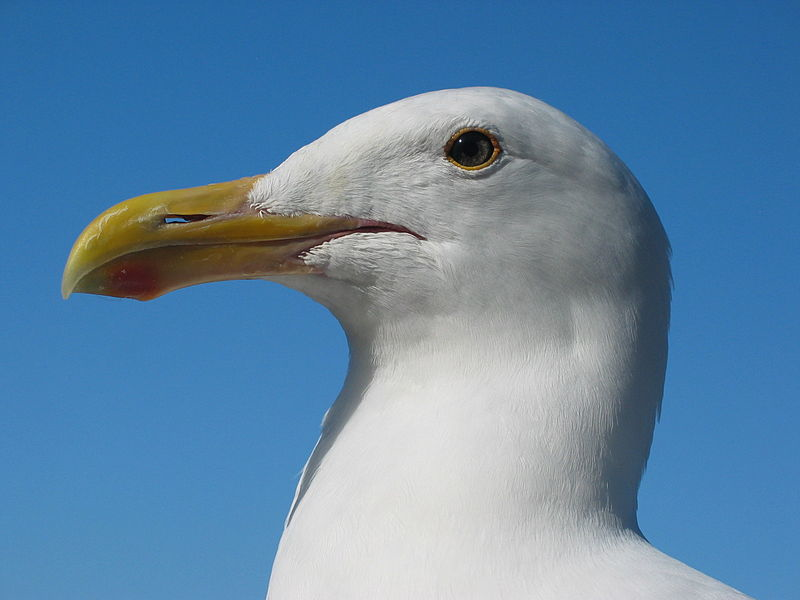
\includegraphics[width=\textwidth]{gull}
    \caption{A gull}
    \label{fig:gull}
  \end{subfigure}%
  ~ %add desired spacing between images, e. g. ~, \quad, \qquad etc.
  % (or a blank line to force the subfigure onto a new line)
  \begin{subfigure}[b]{0.3\textwidth}
    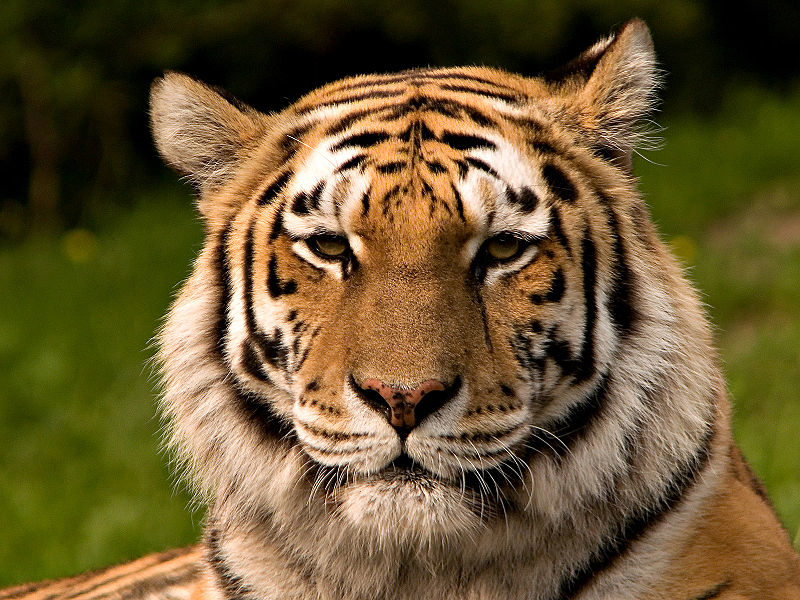
\includegraphics[width=\textwidth]{tiger}
    \caption{A tiger}
    \label{fig:tiger}
  \end{subfigure}
  ~ %add desired spacing between images, e. g. ~, \quad, \qquad etc.
  % (or a blank line to force the subfigure onto a new line)
  \begin{subfigure}[b]{0.3\textwidth}
    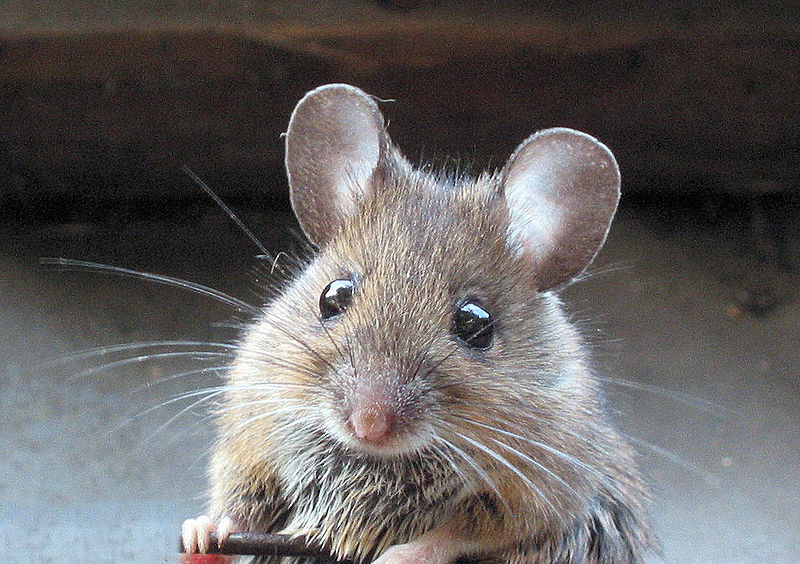
\includegraphics[width=\textwidth]{mouse}
    \caption{A mouse}
    \label{fig:mouse}
  \end{subfigure}
  \caption{Pictures of animals}\label{fig:animals}
\end{figure}

Here is Figure \ref{fig:gull} by itself. Note that the counter in the
figure caption increased (as expected).
\begin{figure}
  \centering
  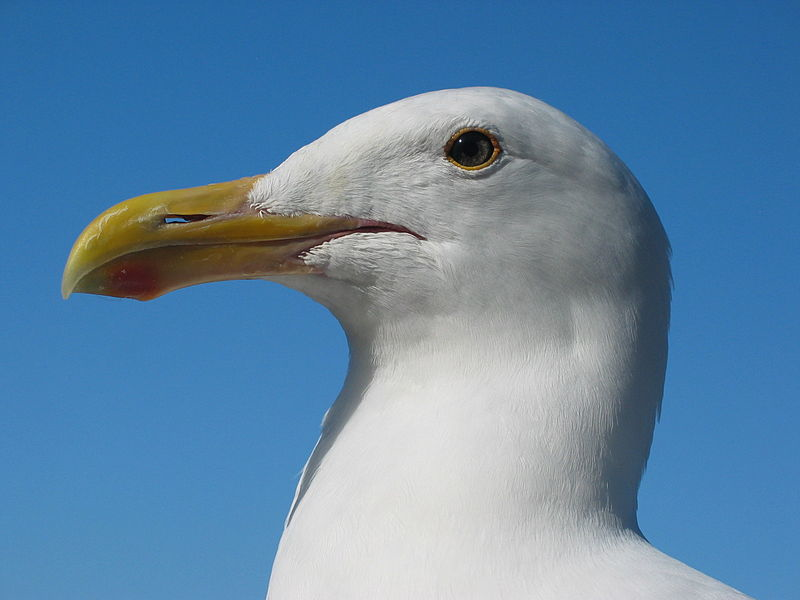
\includegraphics[width=\textwidth]{gull}
  \caption{The gull by itself.}
  \label{fig:gull_alone}
\end{figure}

\section{TikZ Image}
\emph{TikZ} is a popular \LaTeX package for technical drawings.
The following graph shows one of the
\href{http://www.texample.net/tikz/examples/j-curve}{publicly
  available} examples.
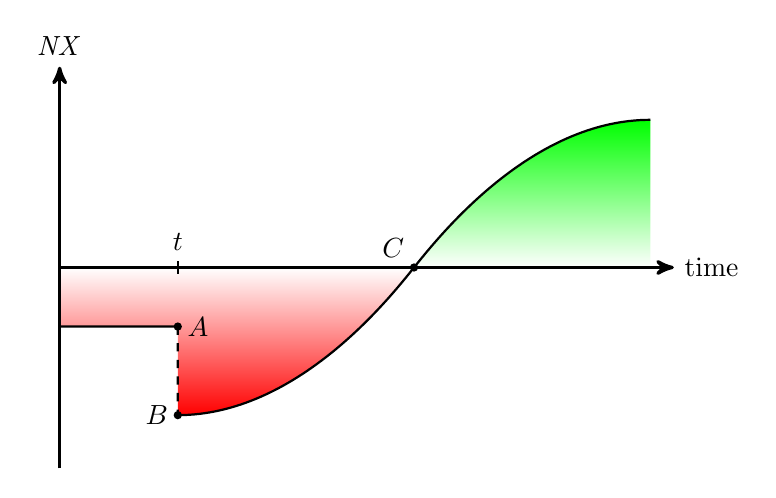
\begin{tikzpicture}[
        %We set the scale and define some styles
        scale=1.5,
        axis/.style={very thick, ->, >=stealth'},
        important line/.style={thick},
        dashed line/.style={dashed, thick},
        every node/.style={color=black,}
     ]
    % Important coordinates are defined
    \coordinate (beg_1) at (0,-.5);
    \coordinate (beg_2) at ($(beg_1)+(1,0)$);
    \coordinate (dev_1) at ($(beg_2)+(0,-.75)$);
    \coordinate (xint) at (3,0);
    \coordinate (end) at (5,1.25);

    %We make some nice shading to annotate different parts of the curve
    % Everything for x<0
    \begin{scope}
        \shade[top color=white, bottom color=red]
            ($(beg_2)+(0,.5)$) parabola bend (dev_1) (xint)
            (0,0) rectangle (beg_2);
    \end{scope}
    %  Everything for x>0
    \begin{scope}
        \shade[bottom color=white, top color=green]
            (xint) parabola bend (end) ($(end)+(0,-1.25)$);
    \end{scope}
    % axis
    \draw[axis] (0,0)  -- (5.2,0) node(xline)[right] {time};
    \draw[axis] (0,-1.7) -- (0,1.7) node(yline)[above] {$\mathit{NX}$};
    % J curve is drawn
    \draw[important line]
        (beg_1) -- (beg_2)
        (dev_1) parabola (xint)
        (xint) parabola[bend at end] (end);
    % coordinates are added
    \fill[black] (beg_2) circle (1pt) node[right] {$A$};
    \fill[black] (dev_1) circle (1pt) node[left] {$B$};
    \fill[black] (xint) circle (1pt) node[above left] {$C$};
    % The time of the devaluation is added
    \draw[dashed line] (beg_2) -- (dev_1);
    \draw[thick] (1,-1.5pt) -- (1,1.5pt) node[above] {$t$};
\end{tikzpicture}

The end.
\end{document}
